\chapter{Tables}\label{app:tables}
%!TEX root = main.tex

\section{Credible Intervals for Standard Normal Distribution}\label{sec:normal_table}
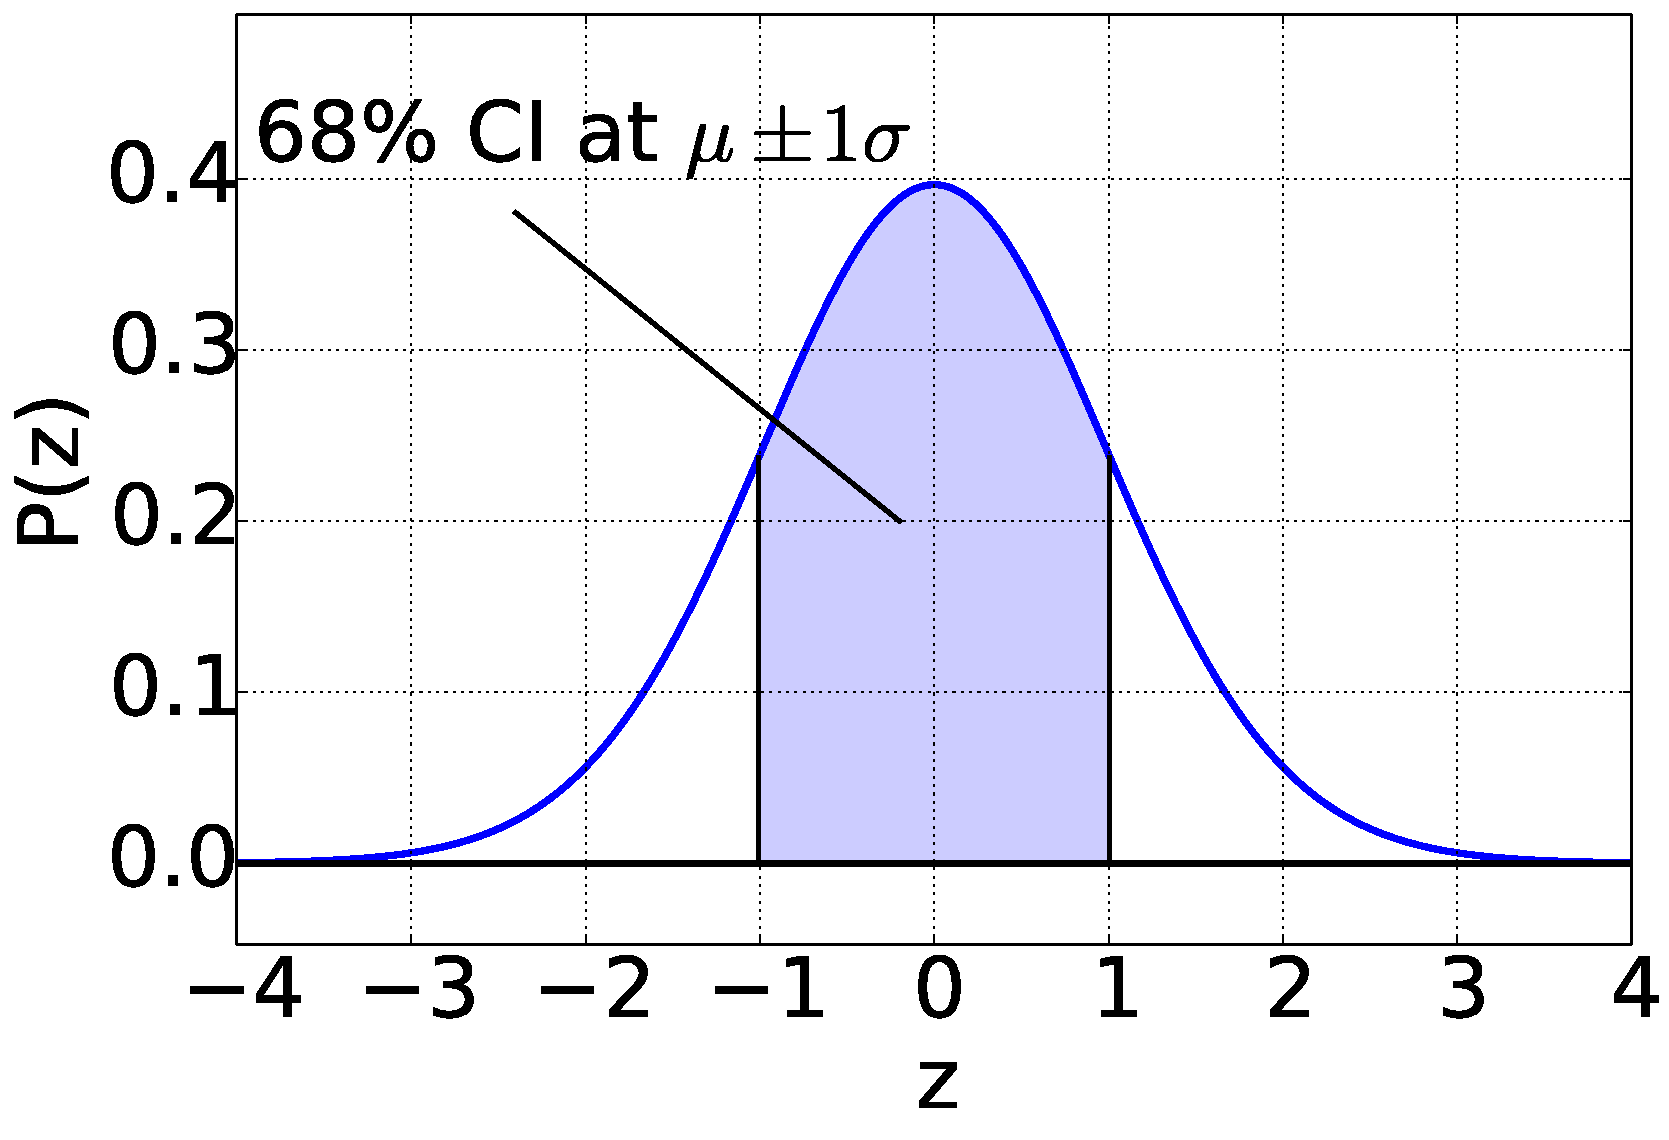
\includegraphics{z_table_CI}

\input z_table_CI.tex

\example{Usage of the Credible Interval Table for the Normal Distribution}

Given a set of 10 samples with sample mean $\bar{x}=5.2$ and known deviation $\sigma=0.3$, the best estimate for the mean parameter $\mu$, representing the true value of the data, is the sample mean, $\hat{\mu}=5.2$ with uncertainty $\sigma/\sqrt{N}$ or $0.3/\sqrt{10}=0.095$.  Some of the credible intervals for this estimate then are the following
\bi
\i 68\% - $[5.2-0.9945 \cdot 0.095, 5.2+0.9945 \cdot 0.095] = [5.11, 5.29]$
\i 95\% - $[5.2-1.9600 \cdot 0.095, 5.2+1.9600 \cdot 0.095] = [5.01,5.39]$
\i 99.8\% - $[5.2-3.0902 \cdot 0.095, 5.2+3.0902 \cdot 0.095] = [4.91,5.49]$
\ei
or approximately
\bi
\i 68\% - $[5.2-1 \cdot 0.095, 5.2+1 \cdot 0.095] = [5.11, 5.29]$
\i 95\% - $[5.2-2 \cdot 0.095, 5.2+2 \cdot 0.095] = [5.01,5.39]$
\i 99.8\% - $[5.2-3 \cdot 0.095, 5.2+3 \cdot 0.095] = [4.91,5.49]$
\ei


\section{Credible Intervals for Student's $t$ Distribution}\label{sec:tdist_table}

\input t_table_CI.tex

\example{Usage of the Credible Interval Table for the Student's $t$ Distribution}

Given a set of 10 samples (9 degrees of freedom) with sample mean $\bar{x}=5.2$ and sample deviation $s=0.3$, the best estimate for the mean parameter $\mu$, representing the true value of the data, is the sample mean, $\hat{\mu}=5.2$ with uncertainty $s/\sqrt{N}$ or $0.3/\sqrt{10}=0.095$.  Some of the credible intervals for this estimate then are the following
\bi
\i 68\% - $[5.2-1.053 \cdot 0.095, 5.2+1.053 \cdot 0.095] = [5.09, 5.3]$
\i 95\% - $[5.2-2.262 \cdot 0.095, 5.2+2.262 \cdot 0.095] = [4.99,5.41]$
\i 99.8\% - $[5.2-4.297 \cdot 0.095, 5.2+4.297 \cdot 0.095] = [4.79,5.61]$
\ei



\newpage
\section{Cumulative Standard Normal Distribution}\label{sec:cumulative_normal_table}

\input z_table.tex
